 % !TEX root = ../report.tex
 
\section{Web app}
This web server has been developed to support the iOS Tinfinity application. 

It is written using Node.js with the Express framework and uses MongoDB as a database. These have been preferred over many alternatives for performance reasons, as they support a very high number of concurrent connections with very little resources. Additionally, websockets are nativly supported using SocketIO, allowing a real-time, bidirectional and reliable chat system.

\begin{figure}[H]
 \makebox[\textwidth][c]{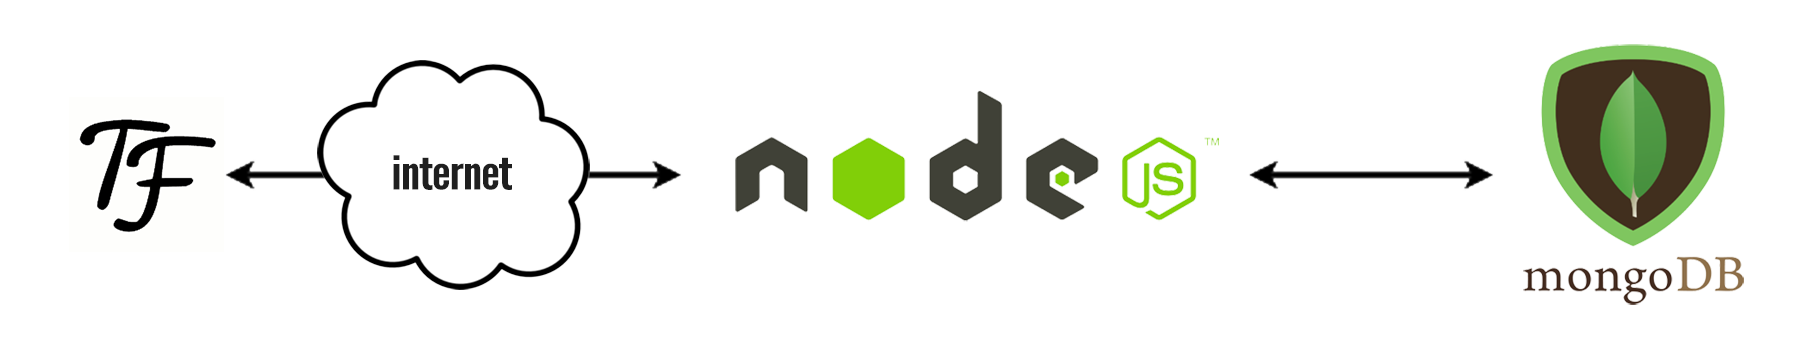
\includegraphics[width=1.0\textwidth]{./images/schema_webapp.png}}%
\caption{Web app overview}
\end{figure}

The structure of the web server has been developed so to not be tightly coupled with the client architecture (iOS), hence other clients (e.g., Web, Android) can be easily created starting from the APIs documentation.

All the security checks are done server-side, not disclosing any unwanted information unless explicitly requested by the user.

MongoDB offers natively Geospatial data type support, and near users are retreived directly querying the database with the user current position.